\documentclass[11pt]{article}
\usepackage[review]{acl}
\usepackage{times}
\usepackage{latexsym}
\usepackage[T1]{fontenc}
\usepackage[utf8]{inputenc}
\usepackage{microtype}
\usepackage{amsmath,amssymb}
\usepackage{booktabs}
\usepackage{multirow}
\usepackage{graphicx}
\usepackage{xcolor}
\newcommand{\SpecVsAgnLHW}{13}
\newcommand{\SpecVsAgnLHL}{5}
\newcommand{\SpecVsAgnLHT}{39}
\newcommand{\SpecVsAgnLHN}{15}
\newcommand{\SpecVsAgnLHC}{57}
\newcommand{\SpecVsAgnLHG}{+14.04}
\newcommand{\DualAgnLHW}{6}
\newcommand{\DualAgnLHL}{2}
\newcommand{\DualAgnLHT}{49}
\newcommand{\DualAgnLHN}{15}
\newcommand{\DualAgnLHC}{57}
\newcommand{\DualAgnLHG}{+7.02}
\newcommand{\DualSpecLHW}{8}
\newcommand{\DualSpecLHL}{5}
\newcommand{\DualSpecLHT}{44}
\newcommand{\DualSpecLHN}{15}
\newcommand{\DualSpecLHC}{57}
\newcommand{\DualSpecLHG}{+5.26}
\newcommand{\DualSpecVsVanLHW}{17}
\newcommand{\DualSpecVsVanLHL}{6}
\newcommand{\DualSpecVsVanLHT}{34}
\newcommand{\DualSpecVsVanLHN}{15}
\newcommand{\DualSpecVsVanLHC}{57}
\newcommand{\DualSpecVsVanLHG}{+19.30}
\newcommand{\CoverLHSpec}{73}
\newcommand{\CoverLHAgn}{16}
\newcommand{\JsdLHSpec}{11.9}
\newcommand{\AgreeLHSpec}{84}
\newcommand{\WeightLHSpec}{0.90}
\newcommand{\TrajLHSpec}{360}
\newcommand{\JsdLHAgno}{6.5}
\newcommand{\AgreeLHAgno}{89}
\newcommand{\WeightLHAgno}{0.94}
\newcommand{\TrajLHAgno}{360}
\newcommand{\SpecVsAgnMTW}{35}
\newcommand{\SpecVsAgnMTL}{21}
\newcommand{\SpecVsAgnMTT}{1}
\newcommand{\SpecVsAgnMTN}{15}
\newcommand{\SpecVsAgnMTC}{57}
\newcommand{\SpecVsAgnMTG}{+2.83}
\newcommand{\DualAgnMTW}{29}
\newcommand{\DualAgnMTL}{27}
\newcommand{\DualAgnMTT}{1}
\newcommand{\DualAgnMTN}{15}
\newcommand{\DualAgnMTC}{57}
\newcommand{\DualAgnMTG}{+0.44}
\newcommand{\DualSpecMTW}{24}
\newcommand{\DualSpecMTL}{28}
\newcommand{\DualSpecMTT}{5}
\newcommand{\DualSpecMTN}{15}
\newcommand{\DualSpecMTC}{57}
\newcommand{\DualSpecMTG}{-1.99}
\newcommand{\DualSpecVsVanMTW}{28}
\newcommand{\DualSpecVsVanMTL}{28}
\newcommand{\DualSpecVsVanMTT}{1}
\newcommand{\DualSpecVsVanMTN}{15}
\newcommand{\DualSpecVsVanMTC}{57}
\newcommand{\DualSpecVsVanMTG}{+0.84}
\newcommand{\CoverMTSpec}{47}
\newcommand{\CoverMTAgn}{1}
\newcommand{\JsdMTSpec}{17.8}
\newcommand{\AgreeMTSpec}{78}
\newcommand{\WeightMTSpec}{0.85}
\newcommand{\TrajMTSpec}{390}
\newcommand{\JsdMTAgno}{19.3}
\newcommand{\AgreeMTAgno}{76}
\newcommand{\WeightMTAgno}{0.84}
\newcommand{\TrajMTAgno}{390}
\newcommand{\SpecVsAgnQAW}{40}
\newcommand{\SpecVsAgnQAL}{17}
\newcommand{\SpecVsAgnQAT}{0}
\newcommand{\SpecVsAgnQAN}{15}
\newcommand{\SpecVsAgnQAC}{57}
\newcommand{\SpecVsAgnQAG}{+0.22}
\newcommand{\DualAgnQAW}{35}
\newcommand{\DualAgnQAL}{22}
\newcommand{\DualAgnQAT}{0}
\newcommand{\DualAgnQAN}{15}
\newcommand{\DualAgnQAC}{57}
\newcommand{\DualAgnQAG}{+0.12}
\newcommand{\DualSpecQAW}{43}
\newcommand{\DualSpecQAL}{14}
\newcommand{\DualSpecQAT}{0}
\newcommand{\DualSpecQAN}{15}
\newcommand{\DualSpecQAC}{57}
\newcommand{\DualSpecQAG}{+0.32}
\newcommand{\DualSpecVsVanQAW}{47}
\newcommand{\DualSpecVsVanQAL}{10}
\newcommand{\DualSpecVsVanQAT}{0}
\newcommand{\DualSpecVsVanQAN}{15}
\newcommand{\DualSpecVsVanQAC}{57}
\newcommand{\DualSpecVsVanQAG}{+0.55}
\newcommand{\CoverQASpec}{34}
\newcommand{\CoverQAAgn}{21}
\newcommand{\JsdQASpec}{14.1}
\newcommand{\AgreeQASpec}{82}
\newcommand{\WeightQASpec}{0.88}
\newcommand{\TrajQASpec}{345}
\newcommand{\JsdQAAgno}{4.0}
\newcommand{\AgreeQAAgno}{92}
\newcommand{\WeightQAAgno}{0.96}
\newcommand{\TrajQAAgno}{345}
\newcommand{\EvHitOneLH}{62}
\newcommand{\EvHitFiveLH}{91}
\newcommand{\EvLexOneLH}{31}
\newcommand{\EvRandOneLH}{10}
\newcommand{\EvSpecLH}{45}
\newcommand{\EvAgnLH}{26}
\newcommand{\EvNLH}{32}
\newcommand{\EvHitOneQA}{24}
\newcommand{\EvHitFiveQA}{86}
\newcommand{\EvLexOneQA}{14}
\newcommand{\EvRandOneQA}{15}
\newcommand{\EvSpecQA}{40}
\newcommand{\EvAgnQA}{48}
\newcommand{\EvNQA}{29}
\newcommand{\AudMTW}{-0.87}
\newcommand{\AudMTE}{-0.16}

\newcommand{\wlt}[3]{#1/#2/#3}
\title{Query-Specific Cartridges with Dual-View JSD Self-Distillation}
\author{Anonymous working draft}
\begin{document}
\maketitle
\begin{abstract}
Cartridges compress a long document into a small trainable KV cache by self-distilling a frozen model on synthetic conversations. We study two changes for the setting where the query is known at test time. First, \emph{query-specific} synthetic data: a 0.6B reranker retrieves evidence for the query and an answer-guided generator turns it into closed-book practice questions. Second, \emph{Dual-View JSD} (DualJSD) self-distillation: every saved trajectory is re-scored by the same frozen model under two views, the bound evidence ($E$) and the whole document ($W$); the student imitates their mixture $M=\tfrac12(P_E+P_W)$ with per-token weight $1-\mathrm{JSD}(P_E,P_W)$. On LongHealth, MTOB and QASPER with Qwen3-4B-Instruct and native KV budgets of 5--20\% of the whole document, query-specific data improves over generic data under identical training, and its practice covers the query and the gold evidence more often. DualJSD changes training targets only where the two views disagree; its paired effect depends on dataset and data source, which we report in full, including cases where it hurts.
\end{abstract}

\section{Introduction}
Reading a long document for every query is expensive; a compact memory trained once per document is cheaper at inference. Cartridges \citep{eyuboglu2025cartridges} learn such a memory as native KV tensors with a frozen backbone, using self-study conversations generated from document chunks. Two limitations matter when the query is available. (i)~\emph{Dilution}: generic self-study spends the small KV budget on content unrelated to the query. (ii)~\emph{The oracle trap}: plain self-distillation copies a single teacher whose context is either a local chunk (missing information) or the whole document (distracted), so the student inherits that teacher's errors.

We address (i) with query-specific data (\S\ref{sec:data}) and (ii) with DualJSD (\S\ref{sec:dualjsd}). Both keep the backbone, attention and KV interface unchanged; neither uses benchmark answers. Figure~\ref{fig:overview} summarizes the pipeline.

\begin{figure*}[t]
\centering
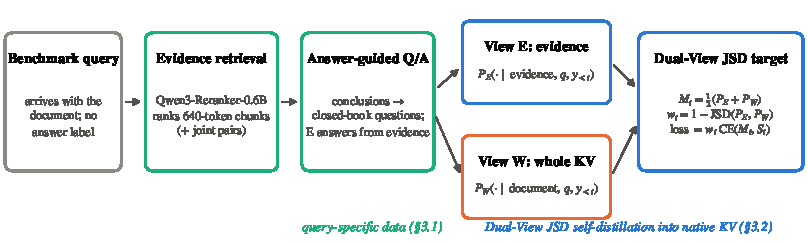
\includegraphics[width=\textwidth]{figures/fig1_overview.pdf}
\caption{Pipeline. Query-specific data binds each synthetic question to reranked evidence; DualJSD mixes the evidence view $E$ and whole-document view $W$ of the same frozen model into a weighted soft target for the native KV student.}
\label{fig:overview}
\end{figure*}

\section{Method}
\subsection{Query-specific synthetic data}\label{sec:data}
The document is split into 640-token chunks. A lexical pre-filter keeps at most 64 chunks; Qwen3-Reranker-0.6B scores each as $P(\texttt{yes}\mid q,\text{chunk})$, then scores 32 entity- or adjacency-linked pairs of the top 16 chunks jointly, yielding up to 32 evidence groups. An answer-guided generator extracts conclusions from an evidence group, writes closed-book questions about them, and a teacher answers from that evidence alone. We keep 15 complete trajectories per request; the agnostic control uses 15 self-study trajectories from the same document.

\subsection{Dual-View JSD self-distillation}\label{sec:dualjsd}
For a saved trajectory with question $q$ and answer tokens $y_{1:T}$ (never regenerated), we teacher-force the frozen model twice: $P_{E,t}=p(\cdot\mid \text{evidence}, q, y_{<t})$, where the evidence is the trajectory's own teacher context (for agnostic data, its self-study chunk), and $P_{W,t}=p(\cdot\mid \text{document}, q, y_{<t})$, using the same native-window head/tail retention as the Whole-KV baseline. On the union of both top-20 supports plus one rest bucket,
\begin{align}
M_t &= \tfrac12\,(P_{E,t}+P_{W,t}),\\
w_t &= 1-\big[H(M_t)-\tfrac12 H(P_{E,t})-\tfrac12 H(P_{W,t})\big]_{\text{bits}},\\
\mathcal{L} &= \textstyle\sum_t w_t\,\mathrm{CE}(M_t, S_t),
\end{align}
where $S_t$ is the student's distribution with the trainable KV. When the views agree, $w_t\approx 1$ and the target is ordinary SD. When one view is uncertain and the other confident, $M_t$ moves toward the confident view. When both are confident but disagree, $w_t\to 0$ and the token is not learned. Everything else---sampler, Adam, learning rate, update budget and the training-loss stopping rule---is identical to SD, so DualJSD differs from SD only in its targets.

\paragraph{What is guaranteed.} For any token $y$, $M_t(y)\ge \tfrac12 \max(P_{E,t}(y),P_{W,t}(y))$, so $-\log_2 M_t(y)$ is at most one bit worse than either view and, by Jensen, no worse than their average. This bounds the \emph{target}; it does not guarantee that a small student exceeds either view, because $E$ and $W$ are the same model and their errors correlate.

\section{Experimental setup}
Qwen3-4B-Instruct-2507, frozen. LongHealth (accuracy), MTOB Kalamang$\to$English (chrF) and QASPER (reference log-perplexity, lower is better). Native KV budgets are 5/10/15/20\% of the measured Whole-KV prefix. All Cartridge arms share the request's initialization, seed, 15 trajectories, learning rate 0.04, accumulated batch 4, at most 32 updates and the same training-loss plateau rule; arms are compared \emph{cell by cell} on identical requests and budgets. Baselines: Whole KV (full document in context), Evidence Teacher (evidence only, no compression), SnapKV at the same byte budget. FastKV (attention matching) at the same budgets is running and not yet included. LongHealth predictions are re-scored by one unique-option extractor.

\section{Results}
\begin{table*}[t]
\centering\small\setlength{\tabcolsep}{4pt}
\resizebox{\textwidth}{!}{\begin{tabular}{llrrrrrrrrr}
\toprule
 & Budget & $n$ & Whole KV & Evid.\ ICL & SnapKV & FastKV (AM) & Vanilla Cart. & Vanilla+DualJSD & Spec.+SD & Spec.+DualJSD (ours) \\
\midrule
\multirow{4}{*}{\shortstack[l]{LongHealth Acc.\,$\uparrow$}} & 5\% & 15 & 86.7 & 80.0 & \textbf{86.7} & 60.0 & 33.3 & 40.0 & 53.3 & 60.0 \\
 & 10\% & 14 & 85.7 & 78.6 & \textbf{85.7} & 78.6 & 64.3 & 57.1 & 64.3 & 64.3 \\
 & 15\% & 14 & 85.7 & 78.6 & \textbf{85.7} & 85.7 & 50.0 & 50.0 & 71.4 & 71.4 \\
 & 20\% & 14 & 85.7 & 78.6 & \textbf{85.7} & 85.7 & 42.9 & 71.4 & 57.1 & 71.4 \\
\midrule
\multirow{4}{*}{\shortstack[l]{MTOB chrF\,$\uparrow$}} & 5\% & 15 & 6.0$^\dagger$ & 27.3 & 5.8$^\dagger$ & 4.1$^\dagger$ & 13.9 & 18.6 & \textbf{19.7} & 17.5 \\
 & 10\% & 14 & 6.0$^\dagger$ & 27.7 & 5.7$^\dagger$ & 4.1$^\dagger$ & 17.0 & 17.3 & \textbf{20.0} & 17.1 \\
 & 15\% & 14 & 6.0$^\dagger$ & 27.7 & 5.8$^\dagger$ & 6.4$^\dagger$ & 17.4 & 17.0 & 17.5 & \textbf{18.9} \\
 & 20\% & 14 & 6.0$^\dagger$ & 27.7 & 5.8$^\dagger$ & -- & 17.0 & 13.8 & \textbf{19.2} & 15.0 \\
\midrule
\multirow{4}{*}{\shortstack[l]{QASPER log-PPL\,$\downarrow$}} & 5\% & 15 & 2.77 & 3.76 & 2.82 & 2.75 & 2.02 & 1.90 & 1.83 & \textbf{1.64} \\
 & 10\% & 14 & 2.80 & 3.86 & 2.76 & 2.63 & 1.93 & 1.90 & 1.78 & \textbf{1.57} \\
 & 15\% & 14 & 2.80 & 3.86 & 2.81 & 2.68 & 2.09 & 1.84 & 1.88 & \textbf{1.29} \\
 & 20\% & 14 & 2.80 & 3.86 & 2.77 & 2.60 & 1.97 & 1.89 & 1.62 & \textbf{1.30} \\
\bottomrule
\end{tabular}
}
\caption{Matched results on the cases every listed method completed ($n$ per cell). Bold: best compressed method. $^\dagger$MTOB Whole KV and SnapKV produce garbled text at the 261K-token window (a baseline-pipeline failure: the same context yields coherent distributions in our scorer) and are not valid comparisons. QASPER log-PPL rewards the answer format that trained Cartridges learn from synthetic data, so values below Whole KV partly reflect format adaptation.}
\label{tab:main}
\end{table*}

\begin{figure*}[t]
\centering
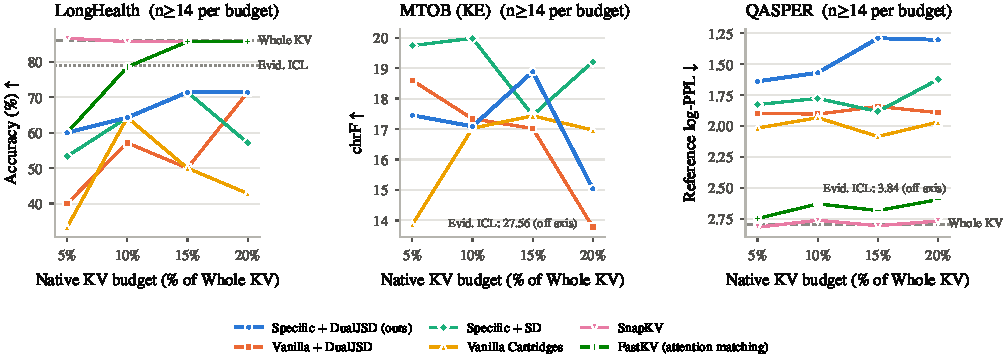
\includegraphics[width=\textwidth]{figures/fig2_main_results.pdf}
\caption{Quality versus native KV budget on matched cases. Dashed/dotted lines: Whole KV and Evidence Teacher (no compression). QASPER axis inverted so that up is better.}
\label{fig:main}
\end{figure*}

\subsection{Why query-specific data helps}
Under identical SD, query-specific data beats generic data in paired cells (win/loss/tie over \SpecVsAgnLHC{} cells from \SpecVsAgnLHN{} requests per dataset; gains are signed so that positive is better) on LongHealth (\wlt{\SpecVsAgnLHW}{\SpecVsAgnLHL}{\SpecVsAgnLHT}, mean \SpecVsAgnLHG{} accuracy points), MTOB (\wlt{\SpecVsAgnMTW}{\SpecVsAgnMTL}{\SpecVsAgnMTT}, \SpecVsAgnMTG{} chrF) and QASPER (\wlt{\SpecVsAgnQAW}{\SpecVsAgnQAL}{\SpecVsAgnQAT}, \SpecVsAgnQAG{} log-PPL). Figure~\ref{fig:specific} shows the mechanism. Its practice mentions the query's content terms far more often (recall \CoverLHSpec\% vs.\ \CoverLHAgn\% on LongHealth, \CoverMTSpec\% vs.\ \CoverMTAgn\% on MTOB), countering dilution. The reranker places a gold-evidence chunk first in \EvHitOneLH\% of LongHealth requests (lexical \EvLexOneLH\%, random \EvRandOneLH\%) and within the top five in \EvHitFiveLH\%, so \EvSpecLH\% of query-specific teacher contexts contain gold evidence versus \EvAgnLH\% of generic chunks. On short QASPER papers the advantage in evidence exposure disappears (\EvSpecQA\% vs.\ \EvAgnQA\%), yet query-specific data still lowers log-PPL, consistent with better-targeted questions rather than evidence exposure alone.

\begin{figure*}[t]
\centering
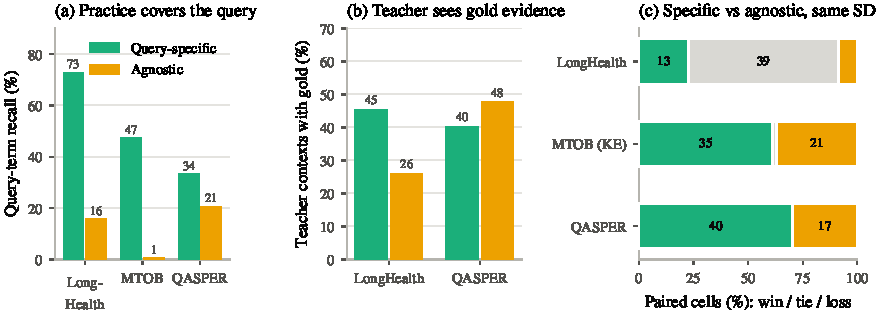
\includegraphics[width=\textwidth]{figures/fig3_query_specific.pdf}
\caption{Why query-specific data helps. (a) Fraction of practice questions sharing a content term with the query. (b) Fraction of the 15 teacher contexts containing annotated gold evidence (labels used only for this audit). (c) Paired cells, specific vs.\ agnostic data under the same SD.}
\label{fig:specific}
\end{figure*}

\subsection{How and when DualJSD helps}
The two views genuinely disagree: on specific data, \JsdLHSpec\%, \JsdMTSpec\% and \JsdQASpec\% of answer tokens have JSD $>0.3$ on LongHealth, MTOB and QASPER, and $W$ assigns lower probability to $E$'s own answers (Figure~\ref{fig:dualjsd}b), i.e.\ the whole-document view softens confident evidence-only predictions. Paired against SD on the same data, DualJSD on specific data wins \wlt{\DualSpecQAW}{\DualSpecQAL}{\DualSpecQAT} cells on QASPER (mean \DualSpecQAG{} log-PPL) and \wlt{\DualSpecLHW}{\DualSpecLHL}{\DualSpecLHT} on LongHealth (\DualSpecLHG{} points; most cells tie because accuracy over $\sim$4 questions is coarse), but loses on MTOB (\wlt{\DualSpecMTW}{\DualSpecMTL}{\DualSpecMTT}, \DualSpecMTG{} chrF). On agnostic data it gives \wlt{\DualAgnLHW}{\DualAgnLHL}{\DualAgnLHT} on LongHealth (\DualAgnLHG{}), \wlt{\DualAgnQAW}{\DualAgnQAL}{\DualAgnQAT} on QASPER (\DualAgnQAG{}) and is roughly neutral on MTOB (\wlt{\DualAgnMTW}{\DualAgnMTL}{\DualAgnMTT}, \DualAgnMTG{}). Combining both changes, Specific+DualJSD versus Vanilla Cartridges wins \wlt{\DualSpecVsVanLHW}{\DualSpecVsVanLHL}{\DualSpecVsVanLHT} on LongHealth (\DualSpecVsVanLHG{} points) and \wlt{\DualSpecVsVanQAW}{\DualSpecVsVanQAL}{\DualSpecVsVanQAT} on QASPER, while on MTOB it only ties vanilla (\wlt{\DualSpecVsVanMTW}{\DualSpecVsVanMTL}{\DualSpecVsVanMTT}) because DualJSD cancels the gain of specific data there.

\paragraph{Why this pattern.} DualJSD changes the target only where $E$ and $W$ disagree. On QASPER and LongHealth, the evidence view is confident but narrow; mixing in $W$ softens those targets with document-level context, and the student generalizes better to the held-out query. On MTOB, the evidence is a precise grammar or lexicon entry from a 261K-token book; $W$ is much less sure of $E$'s answers (mean answer log-prob \AudMTW{} vs.\ \AudMTE{}), so $M$ dilutes exactly the local detail that translation needs. A natural fix, which we have not tested, is to let the weight depend on which view is confident rather than only on their divergence.

\begin{figure*}[t]
\centering
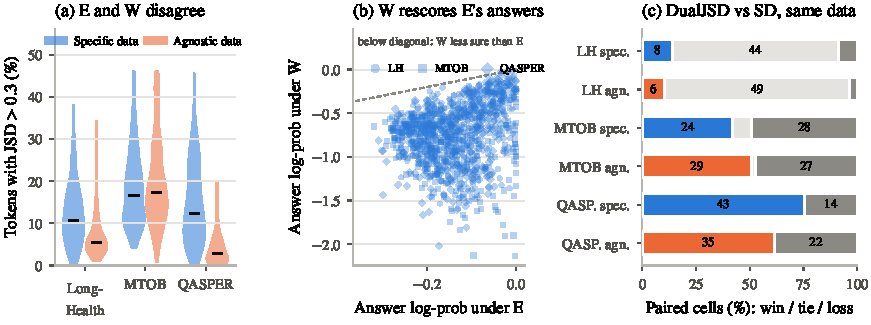
\includegraphics[width=\textwidth]{figures/fig4_dualjsd.pdf}
\caption{DualJSD diagnostics. (a) Per-trajectory share of tokens on which $E$ and $W$ disagree. (b) Mean answer-token log-probability under $E$ vs.\ $W$ (specific data). (c) Paired cells, DualJSD vs.\ SD on the same data.}
\label{fig:dualjsd}
\end{figure*}

\section{Limitations}
Results cover the requests completed within fixed six-hour allocations, ordered by request index rather than sampled at random; cells at different budgets of one request share training targets and are correlated, so the effective sample size is the number of requests. No significance tests are claimed. DualJSD hurts MTOB with specific data. MTOB Whole KV and SnapKV baselines must be re-run; FastKV results are not yet included. QASPER log-PPL partly measures answer-format adaptation. Gold-evidence audits use annotations only for evaluation and exist only for LongHealth and QASPER.

\begin{thebibliography}{1}
\bibitem[{Eyuboglu et~al.(2025)}]{eyuboglu2025cartridges}
Sabri Eyuboglu, Ryan Ehrlich, Simran Arora, Neel Guha, Dylan Zinsley, Emily Liu, Will Tennien, Atri Rudra, James Zou, Azalia Mirhoseini, and Christopher R\'e. 2025.
\newblock Cartridges: Lightweight and general-purpose long context representations via self-study.
\newblock \emph{arXiv preprint arXiv:2506.06266}.
\end{thebibliography}
\end{document}
